\chapter{Datasets}\label{ch:Datasets}


This chapter delves into the datasets employed for experimental validation in this thesis, encompassing real transmission electron microscopy (TEM) and scanning TEM (STEM) images, alongside synthetically generated volumes. It provides comprehensive details on the source, composition, imaging parameters. The utilization of both real and synthetic data is crucial for the effective training, evaluation, and analysis of the proposed methods, ensuring a robust and comprehensive understanding of their performance across diverse data types.


\subsection{TEM Datasets}
    \textbf{Source for all TEM datasets:} CAU Technical Faculty (Synthesis and Real Structure Group)
    
    \begin{itemize}
    \item \textbf{Dataset 1}
    
        This TEM dataset showcases a single nanoparticle image, featuring a range of images with file sizes varying from 20KB to 280KB. Captured at a 20nm scale, these images present a stark contrast with their completely dark background. This dataset provides a diverse array of image qualities, offering a comprehensive view of the nanoparticle across different imaging conditions and resolutions.
        
        \begin{figure}[H]
        \centering
        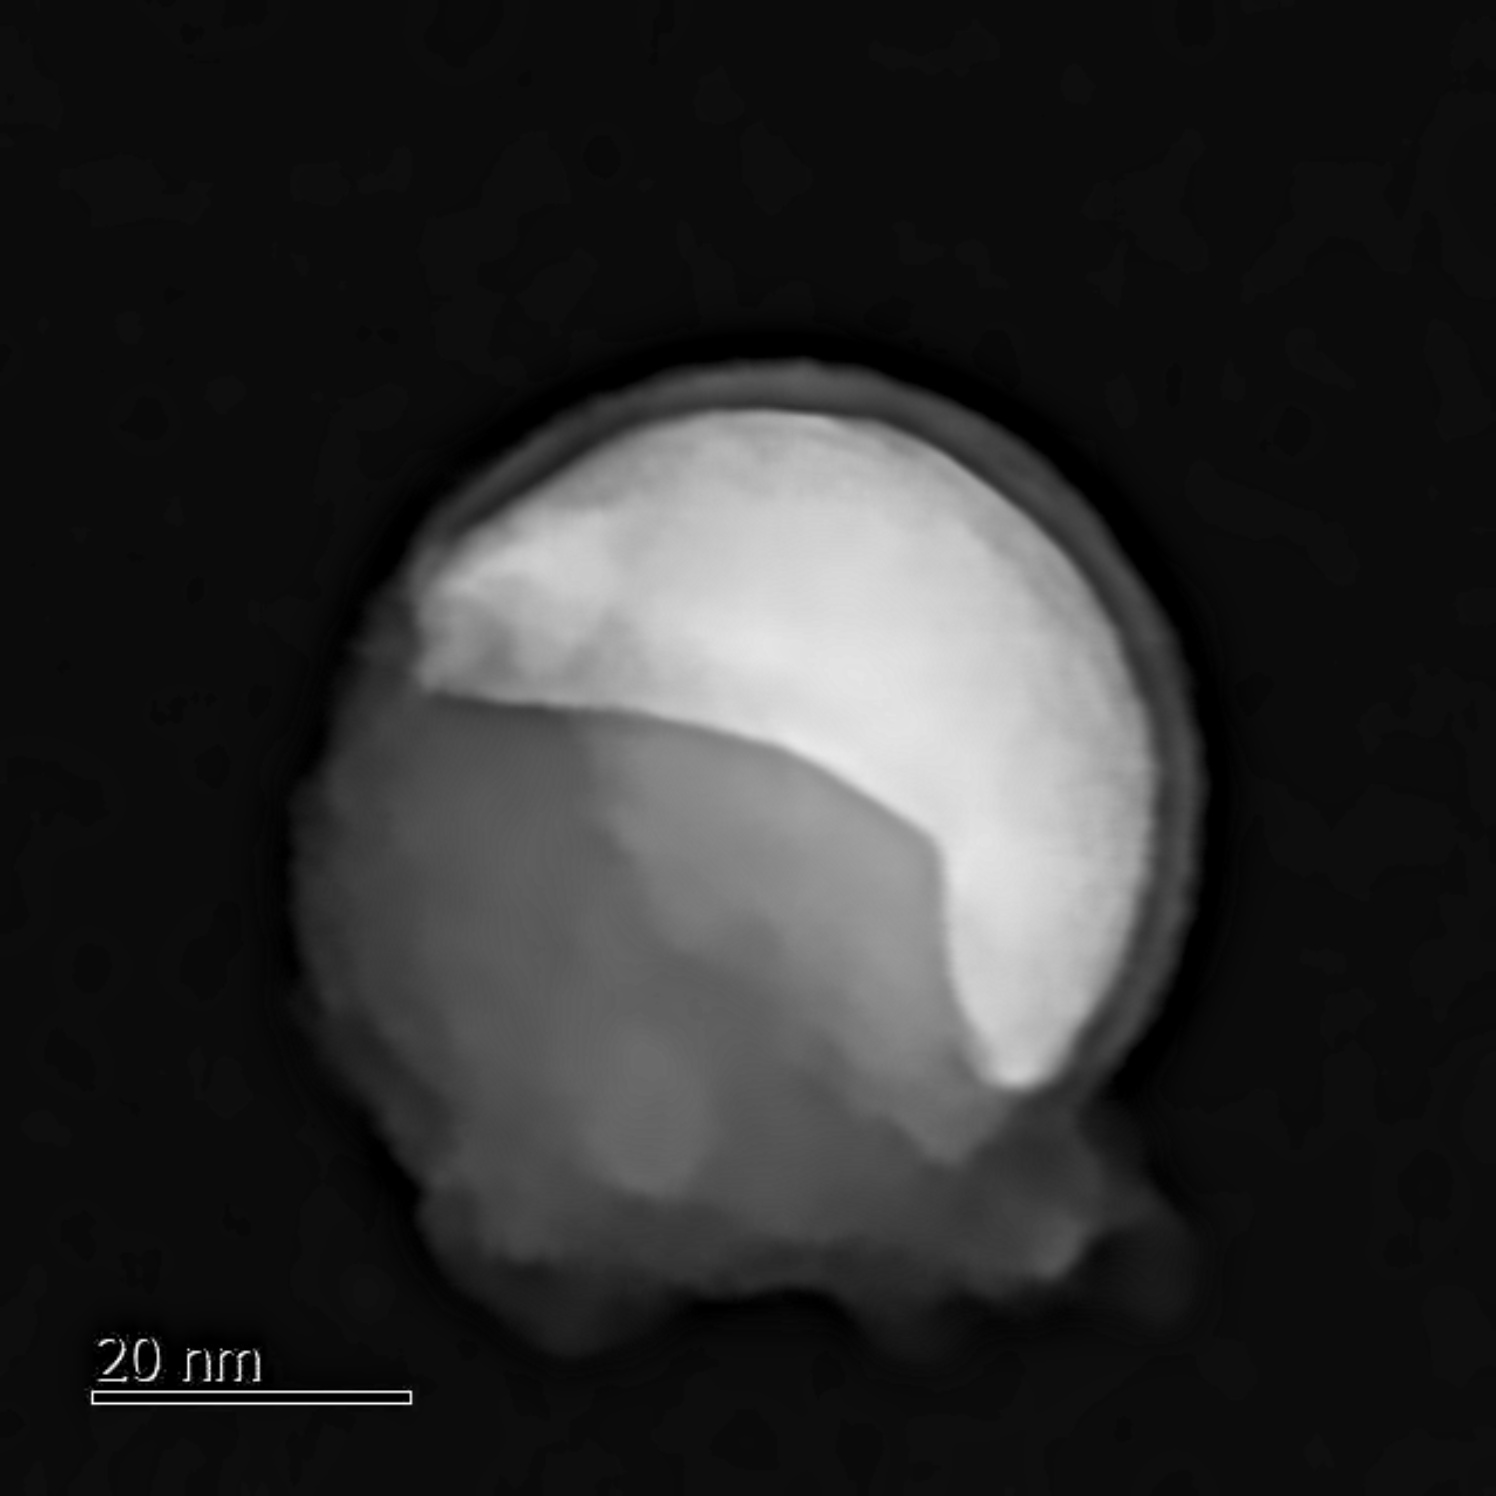
\includegraphics[width=0.4\textwidth]{img/Results/Dataset_1/Single_D1.jpg}
        \caption{Single image from TEM Dataset 1}\label{fig:TEM Dataset 1}
        \end{figure}
        
        \begin{table}[H]
                  \centering
                  \caption{Table Summary: Characteristics of TEM Dataset 1}
                  \begin{tabularx}{.7\linewidth}{|X|X|}
                    \hline
                    \textbf{Total Image} & 10 \\
                    \hline
                    \textbf{Dimensions} & 639 X 639 to  1496 X 1496\\
                    \hline
                    \textbf{Format} & BMP \\
                    \hline
                    \textbf{Image Size} & 20KB to 280KB \\
                    \hline
                  \end{tabularx}
        \end{table}
            
        \begin{figure}[H]
        \centering
        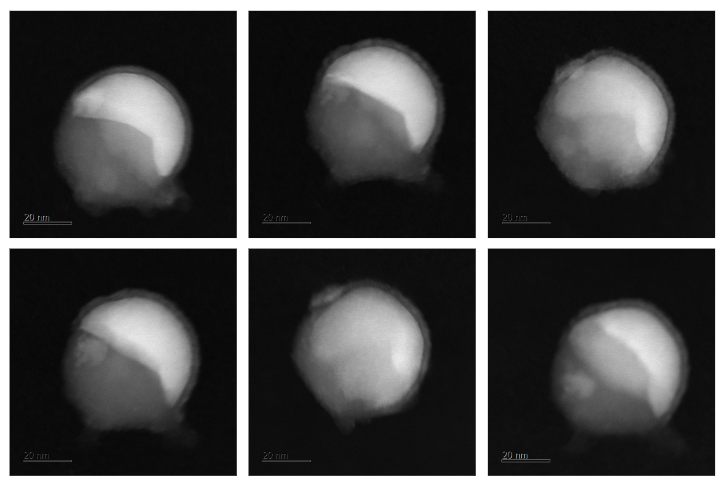
\includegraphics[width=0.71\textwidth]{img/TEM Dataset 1.png}
        \caption{TEM Dataset 1}\label{fig:TEM Dataset 1}
        \end{figure}
        
        To prepare the dataset for NeRF, which requires JPG format, a script converts all BMP images in the folder to JPG. Given the dataset's ten images of varying dimensions, preprocessing is vital to standardizing their shape and aligning all images to the sizes of the first image. This uniformity is crucial for reducing noise and achieving consistent, reliable experiment results.
        \begin{adjustwidth}{0cm}{0cm}
        \begin{listing}[H]
        \begin{minted}[linenos, breaklines, xleftmargin=10pt, xrightmargin=10pt]{python}
        import cv2
        import numpy as np
        
        for idx, file_name in enumerate(grayscale_files):
            grayscale_img = cv2.imread(os.path.join(folder_path, file_name), cv2.IMREAD_GRAYSCALE)
        
            # If it's the first image, store its dimensions
            if idx == 0:
                first_image_height, first_image_width, _ = enhanced_img.shape
        
            enhanced_img = cv2.resize(enhanced_img, (first_image_width, first_image_height))
        \end{minted}
        \caption{Resize all images to match the dimensions of the first image}
        \end{listing}
        
        \end{adjustwidth}


        \item \textbf{Dataset 2}
        
        This TEM dataset features numerous nanoparticles and is more zoomed out at a scale of 200 nm, allowing multiple nanoparticles to be visible in each image. The particles appear white against a completely dark background, making it challenging to discern details with the naked eye. This level of zoom offers a broader view of the sample, but with less detail compared to higher magnification images. 

        \begin{figure}[H]
            \centering
            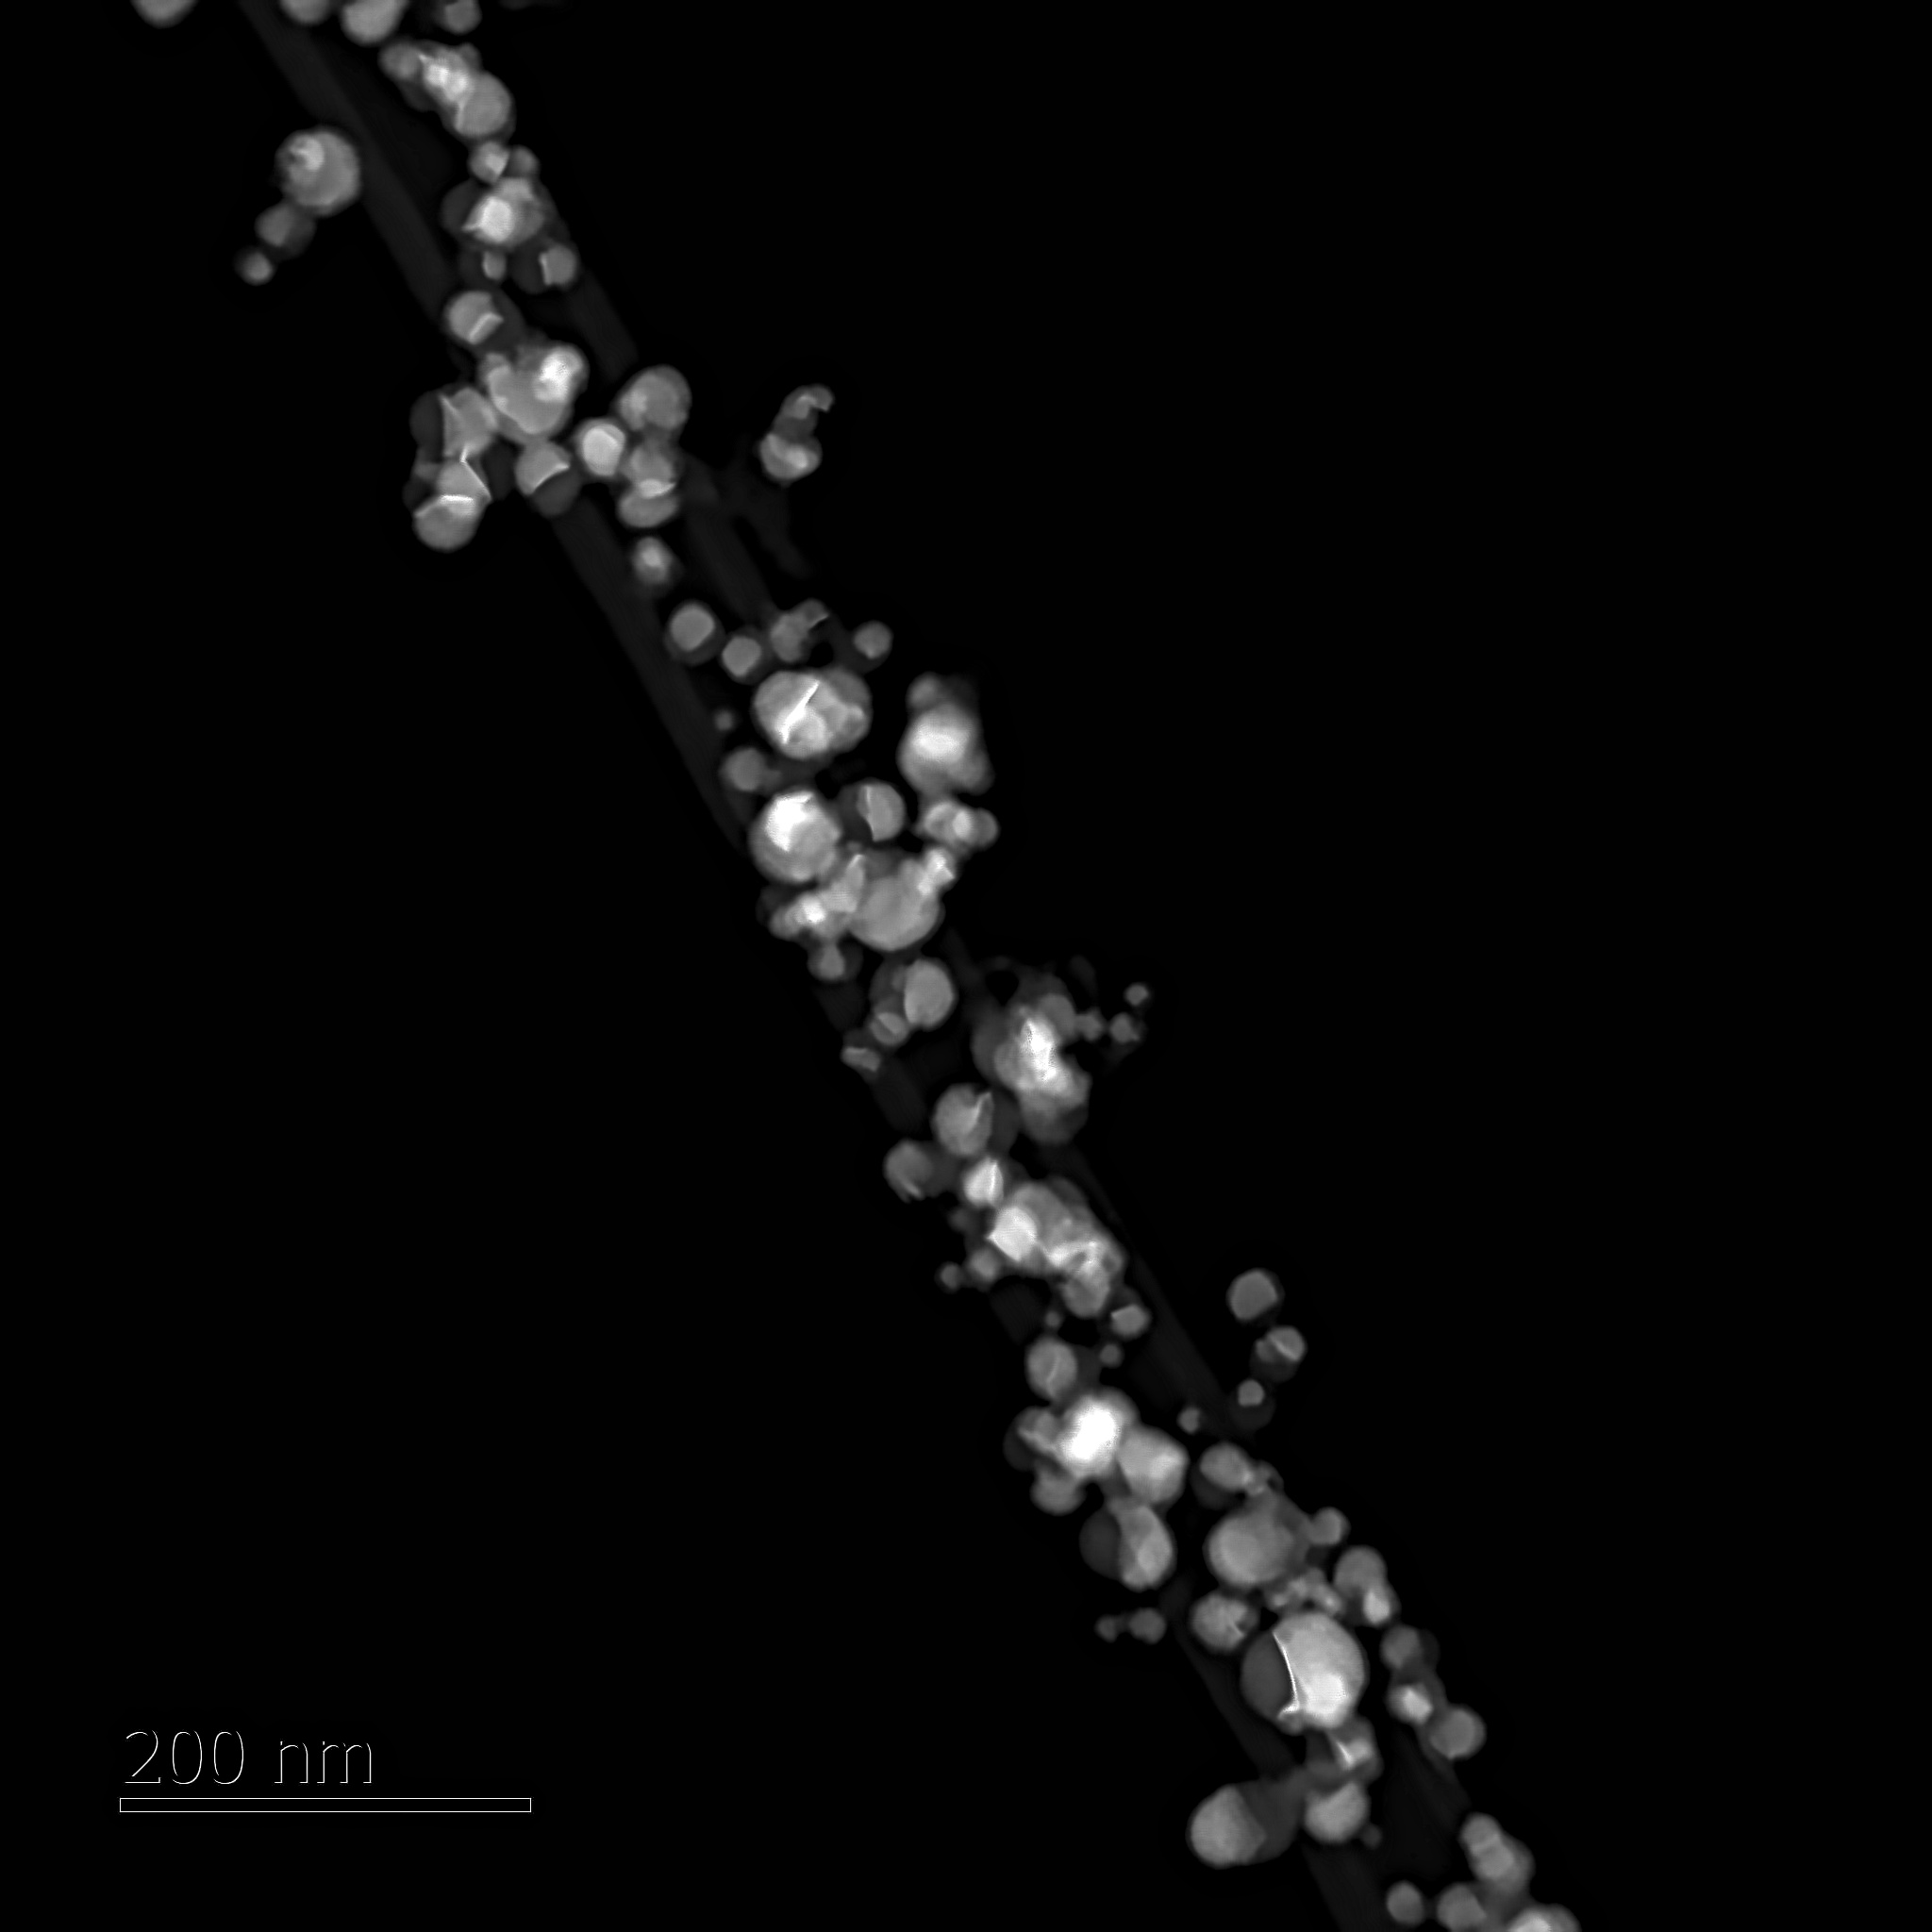
\includegraphics[width=0.4\textwidth]{img/Results/Dataset_2/Single_D2.jpg}
            \caption{Single image from TEM Dataset 2}\label{fig:TEM Dataset 1}
        \end{figure}
        
        \begin{table}[H]
                  \centering
                  \caption{Table Summary: Characteristics of TEM Dataset 2}
                  \begin{tabularx}{.7\linewidth}{|X|X|}
                    \hline
                    \textbf{Total Image} & 23 \\
                    \hline
                    \textbf{Dimensions} & 2048 X 2048\\
                    \hline
                    \textbf{Format} & BMP \\
                    \hline
                    \textbf{Image Size} & 123KB \\
                    \hline
                  \end{tabularx}
              \end{table}
            
        \begin{figure}[H]
        \centering
        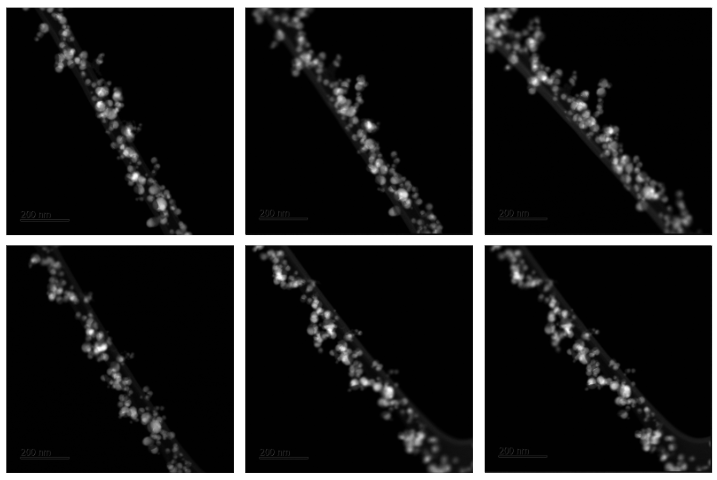
\includegraphics[width=0.71\textwidth]{img/TEM Dataset 2.png}
        \caption{TEM Dataset 2}\label{fig:TEM Dataset 2}
        \end{figure}

       
        % \end{adjustwidth}  
        \vspace{10pt}
        \item \textbf{Dataset 3}


        This dataset features multiple nanoparticles, but lacks specific scale information. The images, clearer than those in other datasets, distinctly show numerous nanoparticles with a V-shaped edge. Despite this clarity, the image quality is moderate with a file size of around 30KB. Notably, the images exhibit considerable noise, affecting the overall visibility and detail of the nanoparticles. This aspect makes it more challenging to analyze and interpret the fine details within the images.

        \begin{figure}[H]
            \centering
            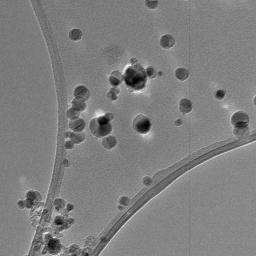
\includegraphics[width=0.4\textwidth]{img/Results/Dataset_3/SIngle_D3.jpg}
            \caption{Single image from TEM Dataset 3}\label{fig:TEM Dataset 1}
        \end{figure}
        
        \begin{table}[H]
                  \centering
                  \caption{Table Summary: Characteristics of TEM Dataset 3}
                  \begin{tabularx}{.7\linewidth}{|X|X|}
                    \hline
                    \textbf{Total Image} & 48 \\
                    \hline
                    \textbf{Dimensions} & 256 X 256\\
                    \hline
                    \textbf{Format} & BMP \\
                    \hline
                    \textbf{Image Size} & 350KB \\
                    \hline
                  \end{tabularx}
              \end{table}
            
        \begin{figure}[H]
        \centering
        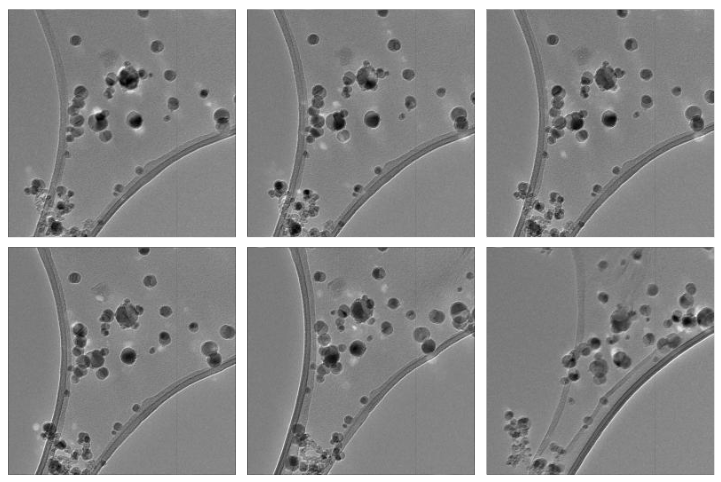
\includegraphics[width=0.71\textwidth]{img/TEM Dataset 3.png}
        \caption{TEM Dataset 3}\label{fig:TEM Dataset 3}
        \end{figure}

        \item \textbf{Dataset 4}

        This dataset, similar in clarity to \ref{fig:TEM Dataset 3}, features numerous nanoparticles. These particles are notably clustered at the top, middle, and bottom sections, forming concentrated groups. The background is gray, with lighter areas around the edges of the images, providing a contrast to the clustered nanoparticles. The unique arrangement and background contrast offer a distinctive view, differentiating it from other datasets and emphasizing the clustered nature of the nanoparticles.

        \begin{figure}[H]
            \centering
            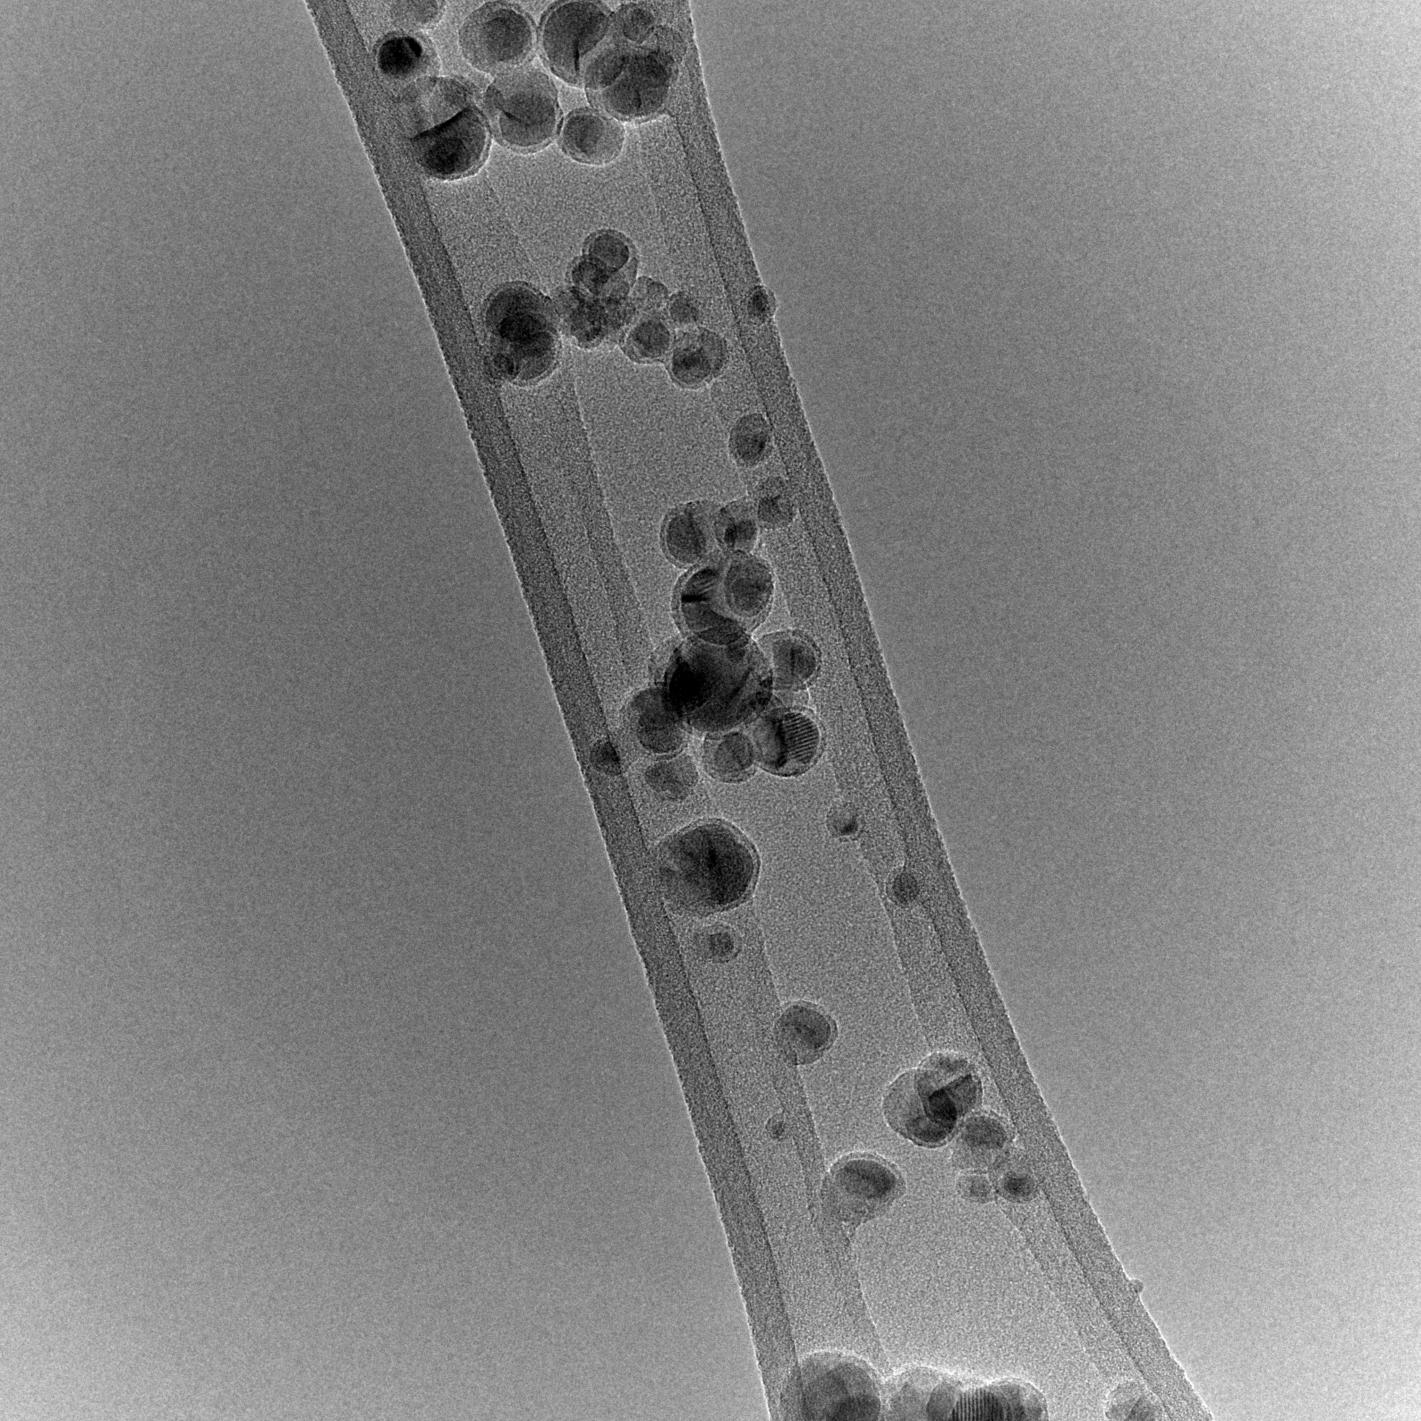
\includegraphics[width=0.4\textwidth]{img/Results/Dataset_4/Single_D4.jpg}
            \caption{Single image from TEM Dataset 4}\label{fig:TEM Dataset 1}
        \end{figure}
        
        \begin{table}[H]
                  \centering
                  \caption{Table Summary: Characteristics of TEM Dataset 4}
                  \begin{tabularx}{.7\linewidth}{|X|X|}
                    \hline
                    \textbf{Total Image} & 20 \\
                    \hline
                    \textbf{Dimensions} & 1421 X 1421\\
                    \hline
                    \textbf{Format} & JPG \\
                    \hline
                    \textbf{Image Size} & 350KB \\
                    \hline
                  \end{tabularx}
              \end{table}
            
        \begin{figure}[H]
        \centering
        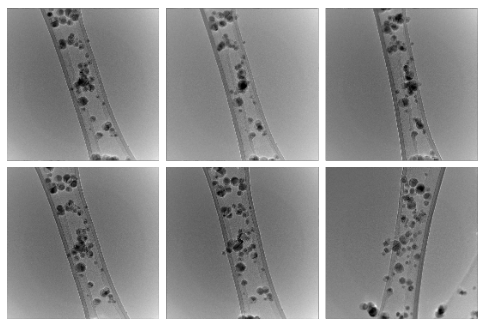
\includegraphics[width=0.71\textwidth]{img/TEM Dataset 4.png}
        \caption{TEM Dataset 4}\label{fig:TEM Dataset 4}
        \end{figure}
    
\end{itemize}
\subsection{STEM Datasets}
    The dataset contains a large, clear particle and a smaller, blurry one, linked by a line. Despite its large 1MB size, the image is unclear and lacks a magnification scale.
    \vspace{5pt}
    
    \textbf{Source for all STEM datasets:} CAU Technical Faculty (Synthesis and Real Structure Group)
    
\begin{itemize}
        \item \textbf{Dataset 1}
        
        \begin{figure}[H]
            \centering
            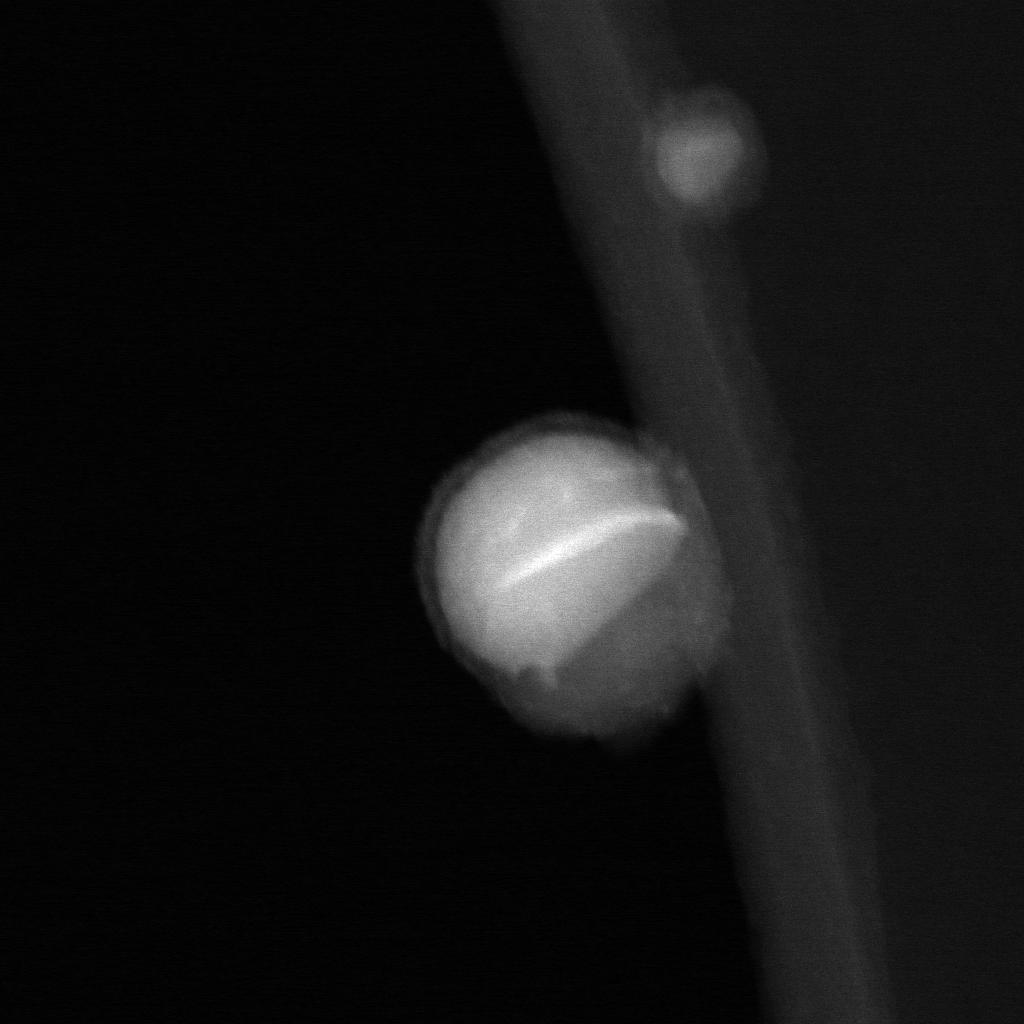
\includegraphics[width=0.4\textwidth]{img/Results/STEM dataset 1/Single_SD1.jpg}
            \caption{Single image from STEM Dataset 1}\label{fig:STEM Dataset 1}
        \end{figure}
        
        \begin{table}[H]
                  \centering
                  \caption{Table Summary: Characteristics of STEM Dataset 1}
                  \begin{tabularx}{.6\linewidth}{|X|X|}
                    \hline
                    \textbf{Total Image} & 17 \\
                    \hline
                    \textbf{Dimensions} & 1024 X 1024\\
                    \hline
                    \textbf{Format} & JPG \\
                    \hline
                    \textbf{Image Size} & 1MB \\
                    \hline
                  \end{tabularx}
              \end{table}
            
        \begin{figure}[H]
        \centering
        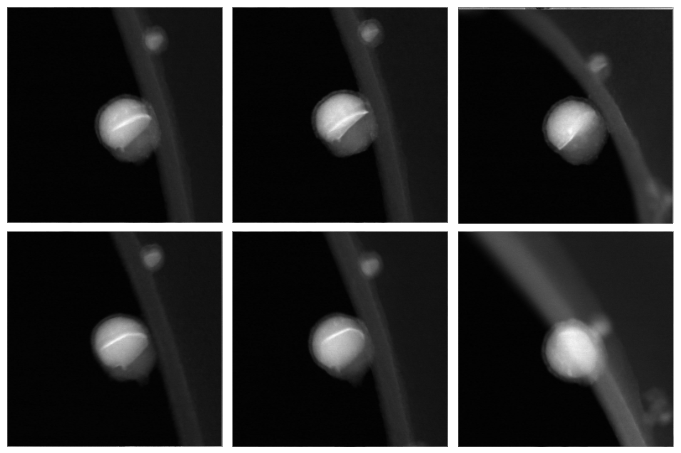
\includegraphics[width=0.62\textwidth]{img/STEM Dataset 1.png}
        \caption{STEM Dataset 1}\label{fig:STEM Dataset 1}
        \end{figure}

        
        \item \textbf{Dataset 2}

        In this dataset, visual inspection reveals a relatively larger nanoparticle centrally positioned, with two smaller, blurry particles in the background. The image quality is notably low, with a file size of only 80KB, making it challenging to discern detailed information about the nanoparticles. The poor clarity and limited size of the image significantly hinder the ability to gain any meaningful insights into the characteristics of these nanoparticles.

        \begin{figure}[H]
            \centering
            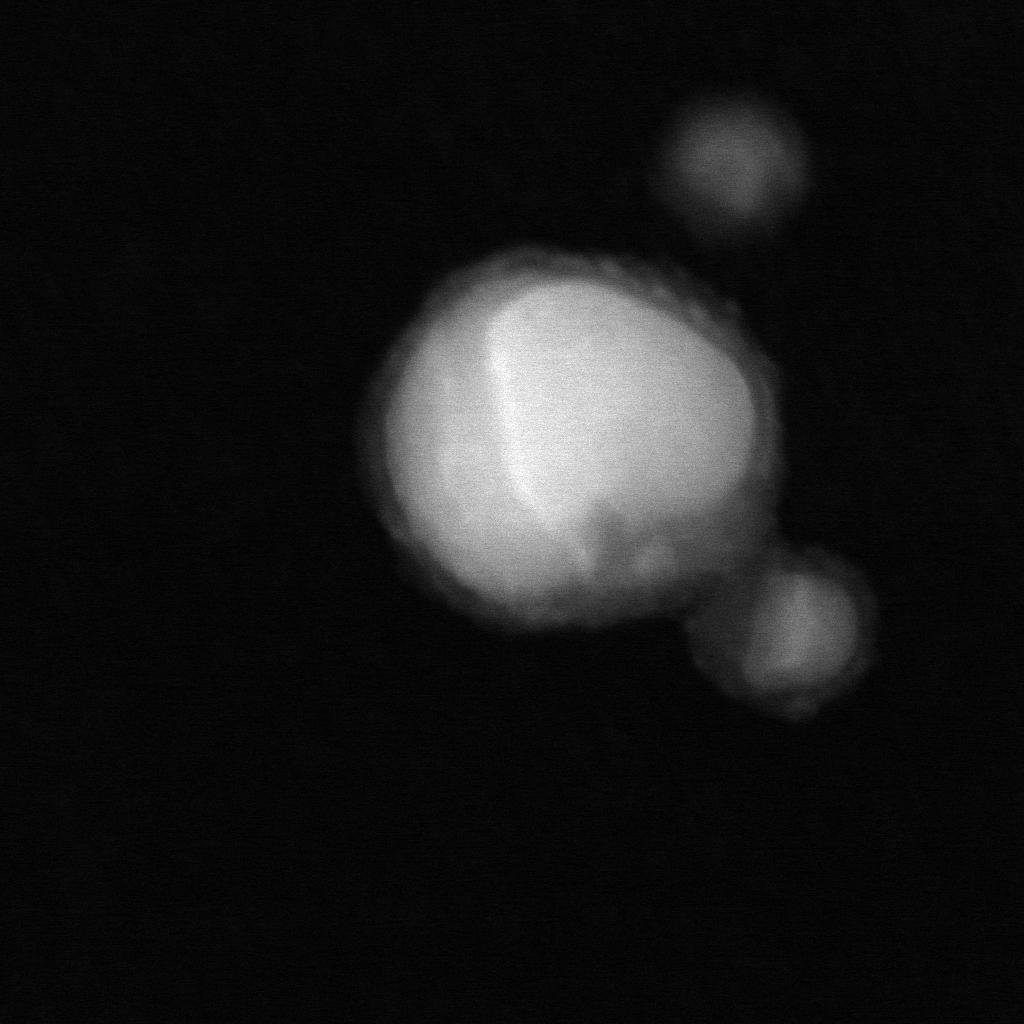
\includegraphics[width=0.4\textwidth]{img/Results/STEM dataset 2/Single_SD2.jpg}
            \caption{Single image from STEM Dataset 2}\label{fig:STEM Dataset 2}
        \end{figure}
        
        \begin{table}[H]
                  \centering
                  \caption{Table Summary: Characteristics of STEM Dataset 2}
                  \begin{tabularx}{.6\linewidth}{|X|X|}
                    \hline
                    \textbf{Total Image} & 16 \\
                    \hline
                    \textbf{Dimensions} & 1024 X 1024\\
                    \hline
                    \textbf{Format} & JPG \\
                    \hline
                    \textbf{Image Size} & 80KB \\
                    \hline
                  \end{tabularx}
              \end{table}
            
        \begin{figure}[H]
        \centering
        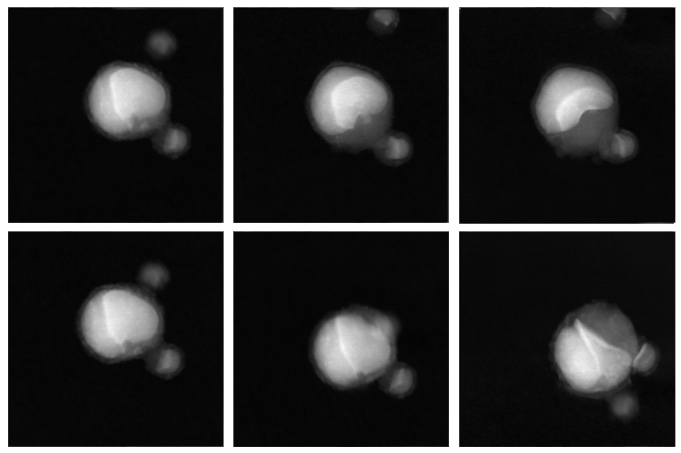
\includegraphics[width=0.7\textwidth]{img/STEM Dataset 2.png}
        \caption{STEM Dataset 2}\label{fig:STEM Dataset 2}
        \end{figure}
    
\end{itemize}
\subsection{Synthetic Dataset}
\begin{itemize}
        \item \textbf{Dataset 1}

        This synthetic dataset, not an actual TEM or STEM dataset, was created using Blender to mimic the appearance of TEM/STEM data from \cite{Rakib2024}. Despite its clarity and lower noise levels, each image is only about 80KB. The collection comprises approximately 120 images, offering a rich perspective from various angles. The dataset features a grey background with light nanoparticle shapes at the center, providing a clear and informative visual representation despite its synthetic origin.

        \begin{figure}[H]
            \centering
            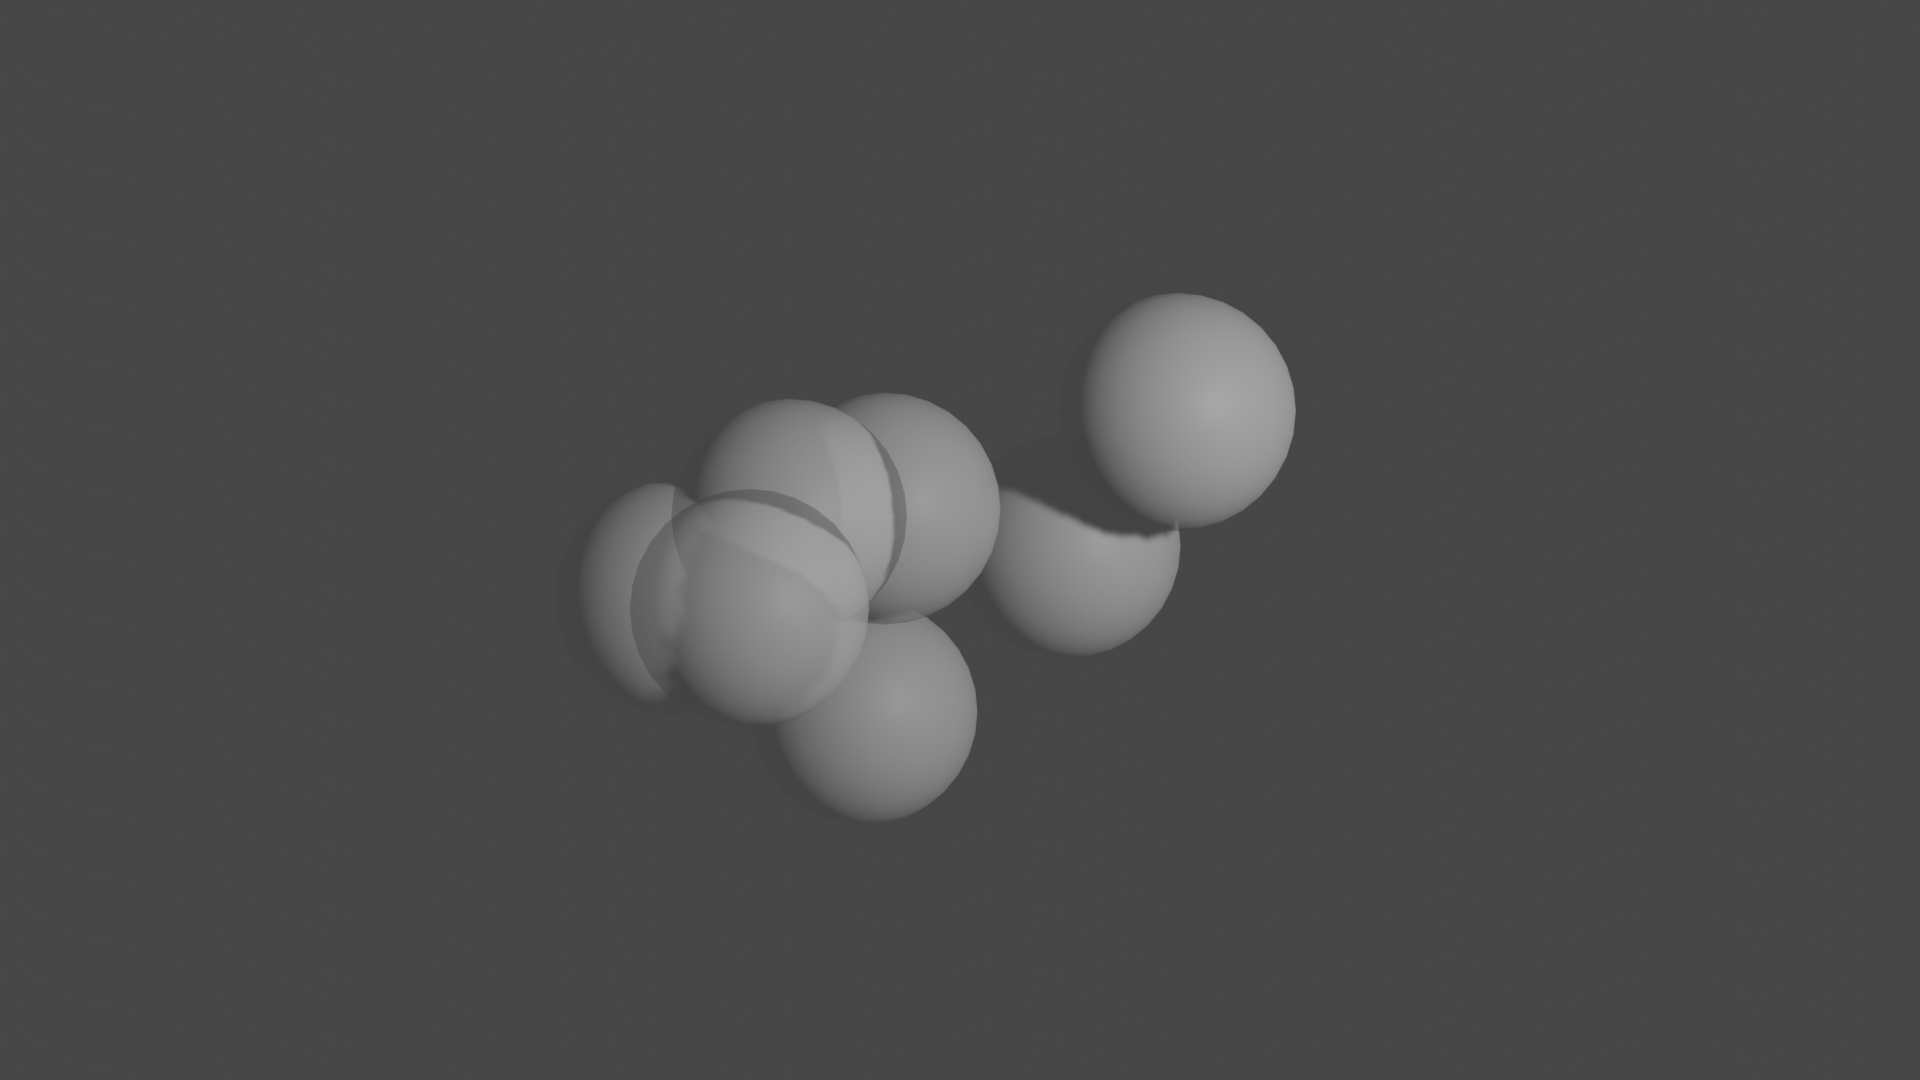
\includegraphics[width=0.6\textwidth]{img/Results/Synthetic data/Single_SYN_D.png}
            \caption{Single image from Synthetic Dataset \cite{Rakib2024}}\label{fig:Synthetic Image}
        \end{figure}
        
        \begin{table}[H]
              \centering
              \caption{Table Summary: Characteristics of Synthetic Dataset}
              \begin{tabularx}{0.7\linewidth}{|X|X|}
                \hline
                \textbf{Source} & Blender Generated Data \\
                \hline
                \textbf{Total Image} & 120 \\
                \hline
                \textbf{Dimensions} & 800 X 800\\
                \hline
                \textbf{Format} & JPG \\
                \hline
                \textbf{Image Size} & 80KB \\
                \hline
              \end{tabularx}
              % \caption{Your table caption goes here.}
              % \label{tab:your_table_label}
         \end{table}
        
        \begin{figure}[H]
        \centering
        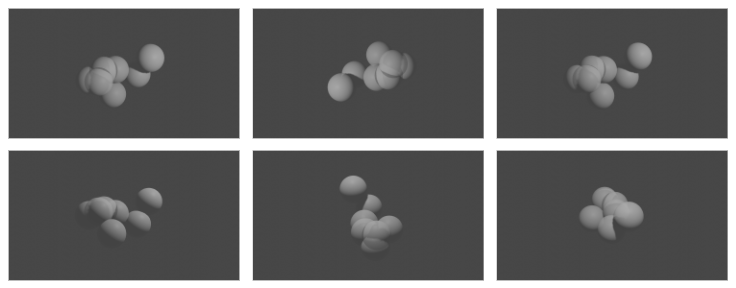
\includegraphics[width=0.71\textwidth]{img/Synthetic Dataset 1.png}
        \caption{Synthetic Dataset \cite{Rakib2024}}\label{fig:Synthetic Dataset}
        \end{figure}
        
\end{itemize}